\chapter{网络层:数据平面}

    \emph{在网络中的每一台主机和路由器中都有一个网络层部分。}

    网络层能够被分解为两个相互作用的部分,即数据平面和控制平面。数据平面功能,即网络层中每台路由器的功能,该数据平面功能决定到达路由器输入链路之一的数据报(即网络层的分组)如何转发到该路由器的输出链路之一。我们将涉及传统的IP转发(其中转发基于数据报的目的地址)和通用的转发(其中可以使用数据报首部中的几个不同域的值执行转发和其他功能)。

    网络层的控制平面功能,即网络范围的逻辑,该控制平面功能控制数据报沿着从源主机到目的主机的端到端路径中路由器之间的路由方式。我们将学习路由选择算法,以及广泛用于今天因特网中的诸如OSPF和BGP等路由选择协议。

\section{网络层概述}

    每台路由器的数据平面的主要作用是从其输入链路向其输出链路转发数据报;控制平面的主要作用是协调这些本地的每路由器转发动作,使得数据报沿着源和目的地主机之间的路由器路径最终进行端到端传送。

\subsection{转发和路由选择:数据平面和控制平面}

    网络层的作用从表现上看就是将分组从一台主机发送到另一台主机。

\begin{itemize}
    \item 转发
    \subitem 当一个分组到达路由器的一条输入链路,该路由器必须将该分组移动到适当的输出链路
    \item 路由选择
    \subitem 分组从发送方刘翔接收方,网络层必须决定这些分组采用的路由或路径。计算这些路径的算法被称为路由选择算法(routing algorithm)
\end{itemize}

    此处,给出较为精确的定义:
    
    转发(forwarding)\emph{指将分组从一个输入链路接口转移到适当的输出链路接口的路由器本地动作。转发发生的时间尺度很短。通常用硬件实现}

    路由选择(routing)\emph{指确定分组从源到目的地所采取的端到端路径的网络范围处理过程。路由选择发生的时间尺度长得多。通常用软件实现}

    每台网络路由器中有一个关键元素是它的转发表(forwarding table)。路由器检査到达分组首部的一个或多个字段值,进而使用这些首部值在其转发表中索引,通过这种方法来转发分组。这些值对应存储在转发表项中的值,指出了该分组将被转发的路由器的输出链路接口

\begin{figure}[!htbp]
    \centering
    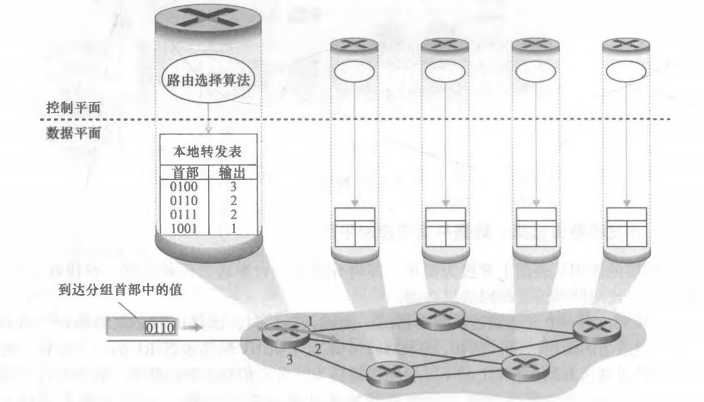
\includegraphics[width=0.8\textwidth]{image/chapter04/路由选择算法.png}
    \caption{路由选择算法决定转发表中的值}
\end{figure}

\subsubsection{控制平面:传统方法}

    路由器中物理上存在的所有转发表的内容是由人类网络操作员直接配置的,进一步说明转发和路由选择功能的区别和不同目的。在这种情况下,不需要任何路由选择协议!当然,这些人类操作员将需要彼此交互,以确保该转发表的配置能使分组到达它们想要到达的目的地。

\subsubsection{控制平面:SDB方法}

    远程控制器计算和分发转发表以供每台路由器所使用。控制平面路由选择功能与物理的路由器是分离的,即路由选择设备仅执行转发,而远程控制器计算并分发转发表。

\begin{figure}[!htbp]
    \centering
    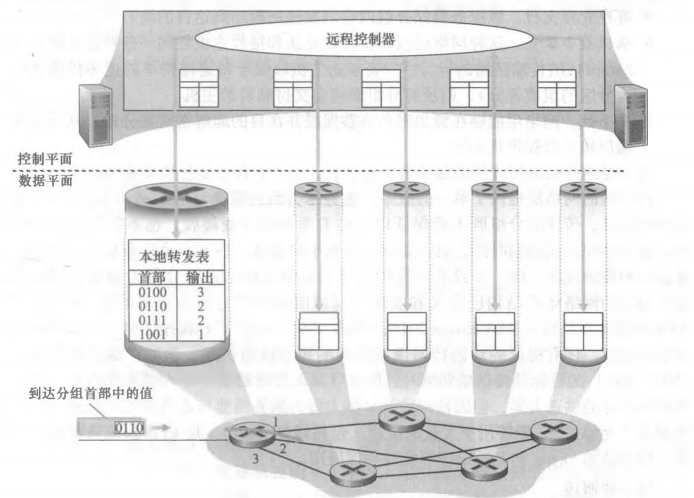
\includegraphics[width=0.6\textwidth]{image/chapter04/远程控制器决定转发表.png}
    \caption{远程控制器确定并分发转发表中的值}
\end{figure}

    显示在图4.2中的控制平面方法是软件定义网络(Software-Defined Networking, SDN)的本质,因为计算转发表并与路由器交互的控制器是用软件实现的,故网络是“软件定义”的。

\subsection{网络服务模型}

    \emph{网络服务模型(network servicemodel)定义了分组在发送与接收端系统之间的端到端运输特性}

    因此,我们考虑网络层能够提供:

\begin{itemize}
    \item 确保交付
    \item 具有时延上界的确保交付
    \item 有序分组交付
    \item 确保最小带宽
    \item 安全性
\end{itemize}

    因特网的网络层提供了单一的服务,称为尽力而为服务(best effort service)。使用尽力而为服务,传送的分组既不能保证以它们发送的顺序被接收,也不能保证它们最终交付;既不能保证端到端时延,也不能保证有最小的带宽。尽力而为服务看起来是根本无服务的一种委婉说法,即一个没有向目的地交付分组的网络也符合尽力而为交付服务的定义!

\section{路由器工作原理}

    我们将注意力转向网络层的转发功能,即实际将分组从一台路由器的入链路传送到适当的出链路

\begin{figure}[!htbp]
    \centering
    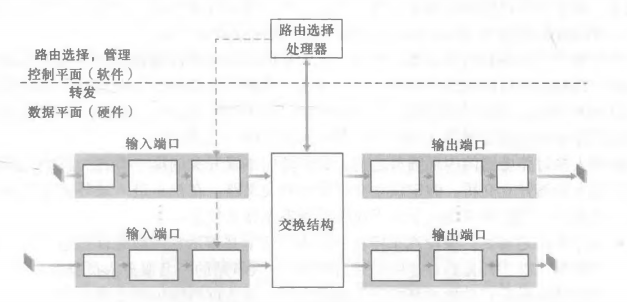
\includegraphics[width=0.8\textwidth]{image/chapter04/路由器体系结构.png}
    \caption{路由器体系结构}
\end{figure}    

\begin{itemize}
    \item 输入端口
    \subitem 在路由器中执行终结入物理链路的物理层功能,位于输入端口最左(输出端口最右)
    \subitem 与入链路远端的数据链路层交互执行数据链路层功能,位于输入输出中间
    \subitem 在输入端执行查找功能,位于输入端口最右,正是这里通过查询转发表决定输出端口
    \item 交换结构 
    \subitem 交换结构将路由器的输入端口连接到输出端口,该结构完全包含在路由器中
    \item 输出端口
    \subitem 输出端口存储从交换结构接收的分组,并通过执行必要的链路层和物理层功能在输出链路上传输这些分组。
    \item 路由选择处理器
    \subitem 路由选择处理器执行控制平面功能。在传统的路由器中,它执行路由选择协议维护路由选择表与关联链路状态信息,并为该路由器计算转发表。
    \subitem 在SDN路由器中,路由选择处理器(在其他活动中)负责与远程控制器通信,目的是接收由远程控制器计算的转发表项,并在该路由器的输入端口安装这些表项。路由选择处理器还执行网络管理功能
\end{itemize}

    路由器的输入端口、输出端口和交换结构几乎总是用硬件实现。

\subsection{输入端口处理和基于目的地转发}

    下图显示了一个更详细的输入处理的视图。

\begin{figure}[!htbp]
    \centering
    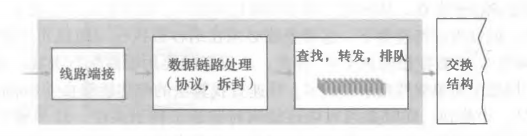
\includegraphics[width=0.6\textwidth]{image/chapter04/输入端口处理.png}
    \caption{输入端口处理}
\end{figure}

    在输入端口中执行的查找对于路由器运行是至关重要的。正是在这个地方,路由器使用转发表来查找输出端口,使得到达的分组能经过交换结构转发到该输出端口。

    转发表是由路由选择处理器计算和更新的(使用路由选择协议与其他网络路由器中的路由选择处理器进行交互),或者转发表接收来自远程SDN控制器的内容。转发表从路由选择处理器经过独立总线(例如一个PCI总线)复制到线路卡

    路由器用分组目的地址的前缀(prefix)与该表中的表项进行匹配;如果存在一个匹配项,则路由器向与该匹配项相关联的链路转发分组。\emph{当有多个匹配时,该路由器使用最长前缀匹配规则(longest prefix matching rule);即在该表中寻找最长的匹配项,并向与最长前缀匹配相关联的链路接口转发分组}

    假定转发表已经存在,从概念上讲表査找是简单的,硬件逻辑只是搜索转发表查找最长前缀匹配。但在G比特速率下,这种查找必须在纳秒级执行。

    因此,不仅必须要用硬件执行查找,而且需要对大型转发表使用超出简单线性搜索的技术;快速查找算法的综述能够在[Gupta 2001, Ruiz Sanchez 2011]中找到。同时必须对内存访问时间给予特别关注,这导致用嵌入式片上DRAM和更快的SRAM (用作一种DRAM缓存)内存来设计。实践中也经常使用三态内容可寻址存储器(Tenary Content Address Memory, TCAM)来查找

    一旦通过查找确定了某分组的输出端口,则该分组就能够发送进入交换结构。在某些设计中,如果来自其他输入端口的分组当前正在使用该交换结构,一个分组可能会在进入交换结构时被暂时阻塞。因此,一个被阻塞的分组必须要在输入端口处排队,并等待稍后被及时调度以通过交换结构

\subsection{交换}

    交换结构位于一台路由器的核心部位, 因为正是通过这种交换结构, 分组才能实际地从一个输入端口交换(即转发)到一个输出端口中。交换可以用许多方式完成

\begin{figure}[!htbp]
    \centering
    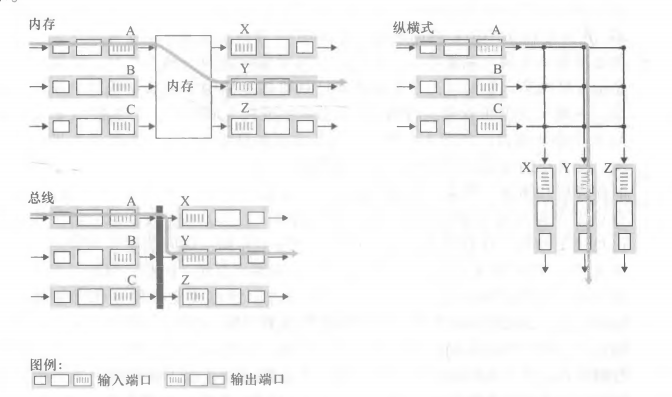
\includegraphics[width=0.6\textwidth]{image/chapter04/三种交换技术.png}
    \caption{三种交换技术}
\end{figure}

\begin{itemize}
    \item 经内存交换
    \subitem 最简单、最早的路由器是传统的计算机,在输入端口与输出端口之间的交换是在CPU(路由选择处理器)的直接控制下完成的。输入与输出端口的功能就像在传统操作系统中的I/O设备一样。
    \subitem 许多现代路由器通过内存进行交换。然而,与早期路由器的一个主要差别是,目的地址的查找和将分组存储(交换)进适当的内存存储位置是由输入线路卡来处理的。在某些方面,经内存交换的路由器看起来很像共享内存的多处理器,用一个线路卡上的处理将分组交换(写)进适当的输出端口的内存中。
    \item 经总线交换
    \subitem 输入端口经一根共享总线将分组直接传送到输出端口,不需要路由选择处理器的干预。
    \subitem 让输入端口为分组预先计划一个交换机内部标签(首部),指示本地输出端口,使分组在总线上传送和传输到输出端口。该分组能由所有输出端口收到,但只有与该标签匹配的端口才能保存该分组。然后标签在输出端口被去除,因为其仅用于交换机内部来跨越总线。
    \item 经互联网络交换
    \subitem 克服单一、共享式总线带宽限制的一种方法是,使用一个更复杂的互联网络。
    \subitem 每条垂直的总线在交叉点与每条水平的总线交叉, 交叉点通过交换结构控制器(其逻辑是交换结构自身的一部分)能够在任何时候开启和闭合。
    \subitem 纵横式交换机是非阻塞的(non-blocking) ,即只要没有其他分组当前被转发到该输出端口,转发到输出端口的分组将不会被到达输出端口的分组阻塞。然而,如果来自两个不同输入端口的两个分组其目的地为根同的输出端口,则一个分组必须在输入端等待,因为在某个时经给定总线仅能发送一个分组
\end{itemize}

\subsection{输出端口处理}

    输出端口处理取出已经存放在输出端口内存中的分组并将其发送到输出链路上。这包括选择和取岀排队的分组进行传输,执行所需的链路层和物理层传输功能

\begin{figure}[!htbp]
    \centering
    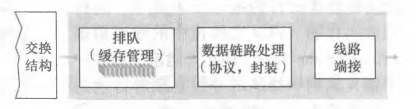
\includegraphics[width=0.8\textwidth]{image/chapter04/输出端口处理.png}
    \caption{输出端口处理}
\end{figure}

\subsection{何处排队}

    在输入端口和输出端口处都可以形成分组队列。排队的位置和程度(或者在输入端口排队,或者在输岀端口排队)将取决于流量负载、交换结构的相对速率和线路速率。

    假定输入线路速度与输出线路速度(传输速率)是相同的,均为$R_{line}$(单位为每秒分组数),并且有N个输入端口和N个输出端口。定义交换结构传送速率$R_{switch}$为从输入端口到输出端口能够移动分组的速率。

\subsubsection{输入排队}

    考虑纵横式交换结构,并假定:
    
\begin{itemize}
    \item [①] 所有链路速度相同;
    \item [②] 一个分组能够以一条输入链路接收一个分组所用的相同的时间量,从任意一个输入端口传送到给定的输出端口
    \item [③] 分组按FCFS方式,从一指定输入队列移动到其要求的输出队列中。
\end{itemize}

    如果位于两个输入队列前端的两个分组是发往同一输出队列的,则其中的一个分组将被阻塞,且必须在输入队列中等待,因为交换结构一次只能传送一个分组到某指定端口。

\begin{figure}[!htbp]
    \centering
    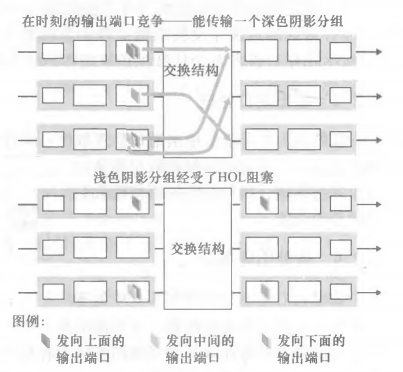
\includegraphics[width=0.6\textwidth]{image/chapter04/输入排队交换机中的HOL阻塞.png}
    \caption{在一个输入排队交换机中的HOL阻塞}
\end{figure}

    左下角队列中的深色阴影分组必须等待。但不仅该分组要等待,左下角队列中排在该分组后面的浅色阴影分组也要等待,即使右中侧输出端口(浅色阴影分组的目的地)中无竞争。

    这种现象叫做输入排毒交换机中的线路前部(Head-Of-the-Line,HOL)阻塞,即在一个输入队列中排队的分组必须等待通过交换结构发送,因为它被位于线路前部的另一个分组阻塞。

\subsubsection{输出排队}

    当没有足够的内存来缓存一个入分组时,就必须做出决定:要么丢弃到达的分组(采用一种称为弃尾(drop tail)的策略),要么删除一个或多个已排队的分组为新来的分组腾出空间。

    在某些情况下,在缓存填满之前便丢弃一个分组(或在其首部加上标记)的做法是有利的,这可以向发送方提供一个拥塞信号。已经提出和分析了许多分组丢弃与标记策略[Labrador 1999, Hollot 2002],这些策略统称为主动队列管理(Active Queue Management ,AQM)算法。随机早期检测(Random Early Detection, RED)算法是得到最广泛研究和实现的AQM算法之一

\begin{figure}[!htbp]
    \centering
    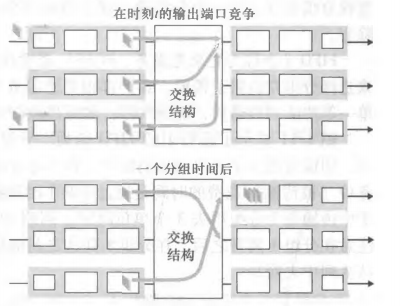
\includegraphics[width=0.6\textwidth]{image/chapter04/输出端口排队.png}
    \caption{输出端口排队}
\end{figure}

    输出端口的分组调度(packet scheduler)在这些排队分组中选择一个分组来传输

\subsection{分组调度}

    现在我们转而讨论确定次序的问题,即排队的分组如何经输出链路传输的问题。

\subsubsection{先进先出}

\begin{figure}[!htbp]
    \centering
    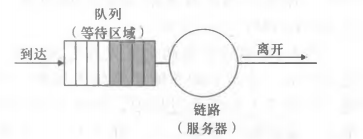
\includegraphics[width=0.6\textwidth]{image/chapter04/FIFO排队抽象.png}
    \caption{FIFO排队抽象}
\end{figure}

    上图显示了对于先进先出(First-In-First-Out, FIFO)链路调度规则的排队模型的抽象。如果链路当前正忙于传输另一个分组,到达链路输出队列的分组要排队等待传输。如果没有足够的缓存空间来容纳到达的分组,队列的分组丢弃策略则确定该分组是否将被丢弃(丢失)或者从队列中去除其他分组以便为到达的分组腾出空间

    